\documentclass[usenames,dvipsnames]{beamer}
%\documentclass[usenames,dvipsnames,handout]{beamer}


\usetheme{AnnArbor}
% \usecolortheme{default}
% \usecolortheme{crane}
\usecolortheme{beaver}
\usecolortheme{dolphin}
% \usecolortheme{orchid}
% \usecolortheme{rose}


\usepackage{fourier}
\usepackage{faktor}
\usepackage{amssymb}
\usepackage{amsmath}
\usepackage{amsthm}
\usepackage{stmaryrd}
\usepackage{hyperref}
\usepackage[all]{xy}
\usepackage[final]{pdfpages}
\usepackage{graphicx}

\newcommand{\downmapsto}{\rotatebox[origin=c]{-90}{$\large\mapsto$}\mkern2mu} %MnSymbol doesn't work well with beamer

\def\Q{\mathbb{Q}}
\def\Z{\mathbb{Z}}
\def\C{\mathbb{C}}
\def\R{\mathbb{R}}
\def\F{\mathbb{F}}

\DeclareMathOperator{\AV}{AV}
%\DeclareMathOperator{\Mat}{Mat}
%\DeclareMathOperator{\Pol}{Pol}
\DeclareMathOperator{\Char}{char}
\DeclareMathOperator{\rk}{Rank}
\DeclareMathOperator{\Frob}{Frob}
\DeclareMathOperator{\ICM}{ICM}
\DeclareMathOperator{\Pic}{Pic}
\DeclareMathOperator{\Aut}{Aut}
\DeclareMathOperator{\End}{End}
\DeclareMathOperator{\Jac}{Jac}
\DeclareMathOperator{\Spec}{Spec}
\DeclareMathOperator{\id}{id}

\newcommand{\cC}{{\mathcal C}}
\newcommand{\cO}{{\mathcal O}}
\newcommand{\cW}{{\mathcal W}}

\newcommand{\p}{{\mathfrak p}}
\newcommand{\frf}{{\mathfrak f}}

\newcommand{\set}[1]{\left\lbrace#1\right\rbrace }

\newcommand{\AVord}[1]{\AV^{\text{ord}}({#1})}
\newcommand{\Modord}[1]{\cM^{\text{ord}}({#1})}

\newcommand{\red}[1]{\textcolor{red}{#1}}
\newcommand{\blue}[1]{\textcolor{blue}{#1}}
\newcommand{\green}[1]{\textcolor{ForestGreen}{#1}}

\newtheorem{df}{Definition}[section]
\newtheorem{remark}[df]{Remark}

%AUTHOR DETAILS
%%%%%%%%%%%%%%%%%%%%%%%%%%%%%%%%%%%%%%%%%%%%%%%%
\title[]{Representing abelian varieties}
\subtitle{}
\author[Stefano Marseglia]{Stefano Marseglia}
\institute[]{Utrecht University}
\date[19 December 2019]{Welcome Home 2019 - Universit\'a di Torino}

% ABSTRACT: 20 minutes
%Abelian varieties are projective varieties whose set of points naturally forms a group. In particular they can be described by equations in some projective space. When the dimension is higher than one, these equations are very cumbersome. In this talk we will give an overview of how can we overcome this difficulty over various fields of definition.

\begin{document}

\begin{frame}
\titlepage
\end{frame}

\begin{frame}{ Abelian Varieties }
\begin{itemize}
 \item An \green{abelian variety} $A$ over a field $k$ is a projective geometrically connected group variety over $k$.\\
 \pause We have \blue{morphisms} $\oplus:A\times A \to A$, $\ominus:A\to A$ and a $k$-rational point $e\in A(k)$ such that $(A,\oplus,\ominus,e)$ is a group object in the category of projective geom.~connected varieties over $k$.
 \pause \item In practice, we have \red{diagrams $\rightsquigarrow$} \blue{``natural'' group structure} on $A(\overline k)$.
 \pause \item eg. ($\ominus$ is the ``inverse'' morphism)
 {\tiny
 \[ 
 	\xymatrix{
 		A\times_k A \ar[rr]^{(\ominus,\id)} 	& 						& A\times_k A \ar[d]^{\oplus}\\
 		A \ar[u]^{\Delta} \ar[r] 	& \Spec(k) \ar[r]^{e}	& A 
 	}
 	\pause \qquad
 	\xymatrix{
 		A\times_k A \ar[rr]^{(\id,\ominus)} 	& 						& A\times_k A \ar[d]^{\oplus}\\
 		A \ar[u]^{\Delta} \ar[r] 	& \Spec(k) \ar[r]^{e}	& A 
 	}
  \]}
\end{itemize}
\end{frame}

\begin{frame}{ Example : $\dim A=1$ elliptic curves  }
\begin{itemize}
	\item AVs of dimension $1$ are called \red{Elliptic Curves}.
	\pause \item They admit a \blue{plane model}: if $\Char k \neq 2,3$
	\[  Y^2Z = X^3 +AXZ^2 + BZ^3\quad A,B \in k\text{ and }e=[0:1:0]  \]
	\pause \item The \green{groups law is explicit}:\\
	if $P=(x_P,y_P) $ then $ \ominus P=(x_P,-y_P) $ and\\
	\pause if $Q=(x_Q,y_Q)\neq \ominus P$ then $P\oplus Q=(x_R,y_R)$ where
	\[ x_R = \lambda^2 -x_P-x_Q, \quad y_R = y_P+\lambda (x_R-x_P), \]
	where
	\[ \lambda = 
	\begin{cases}
		\frac{3x_P^2 + B}{2A}& \text{ if } P=Q  \\
		\frac{y_P -y_Q}{x_P - x_Q} &  \text{ if } P\neq Q
	\end{cases}.
	\]
	
\end{itemize}
\end{frame}

\begin{frame}{ Example : $\dim A=1$ elliptic curves }
In pictures, over $k=\R$:
\begin{figure}[h]
\centering
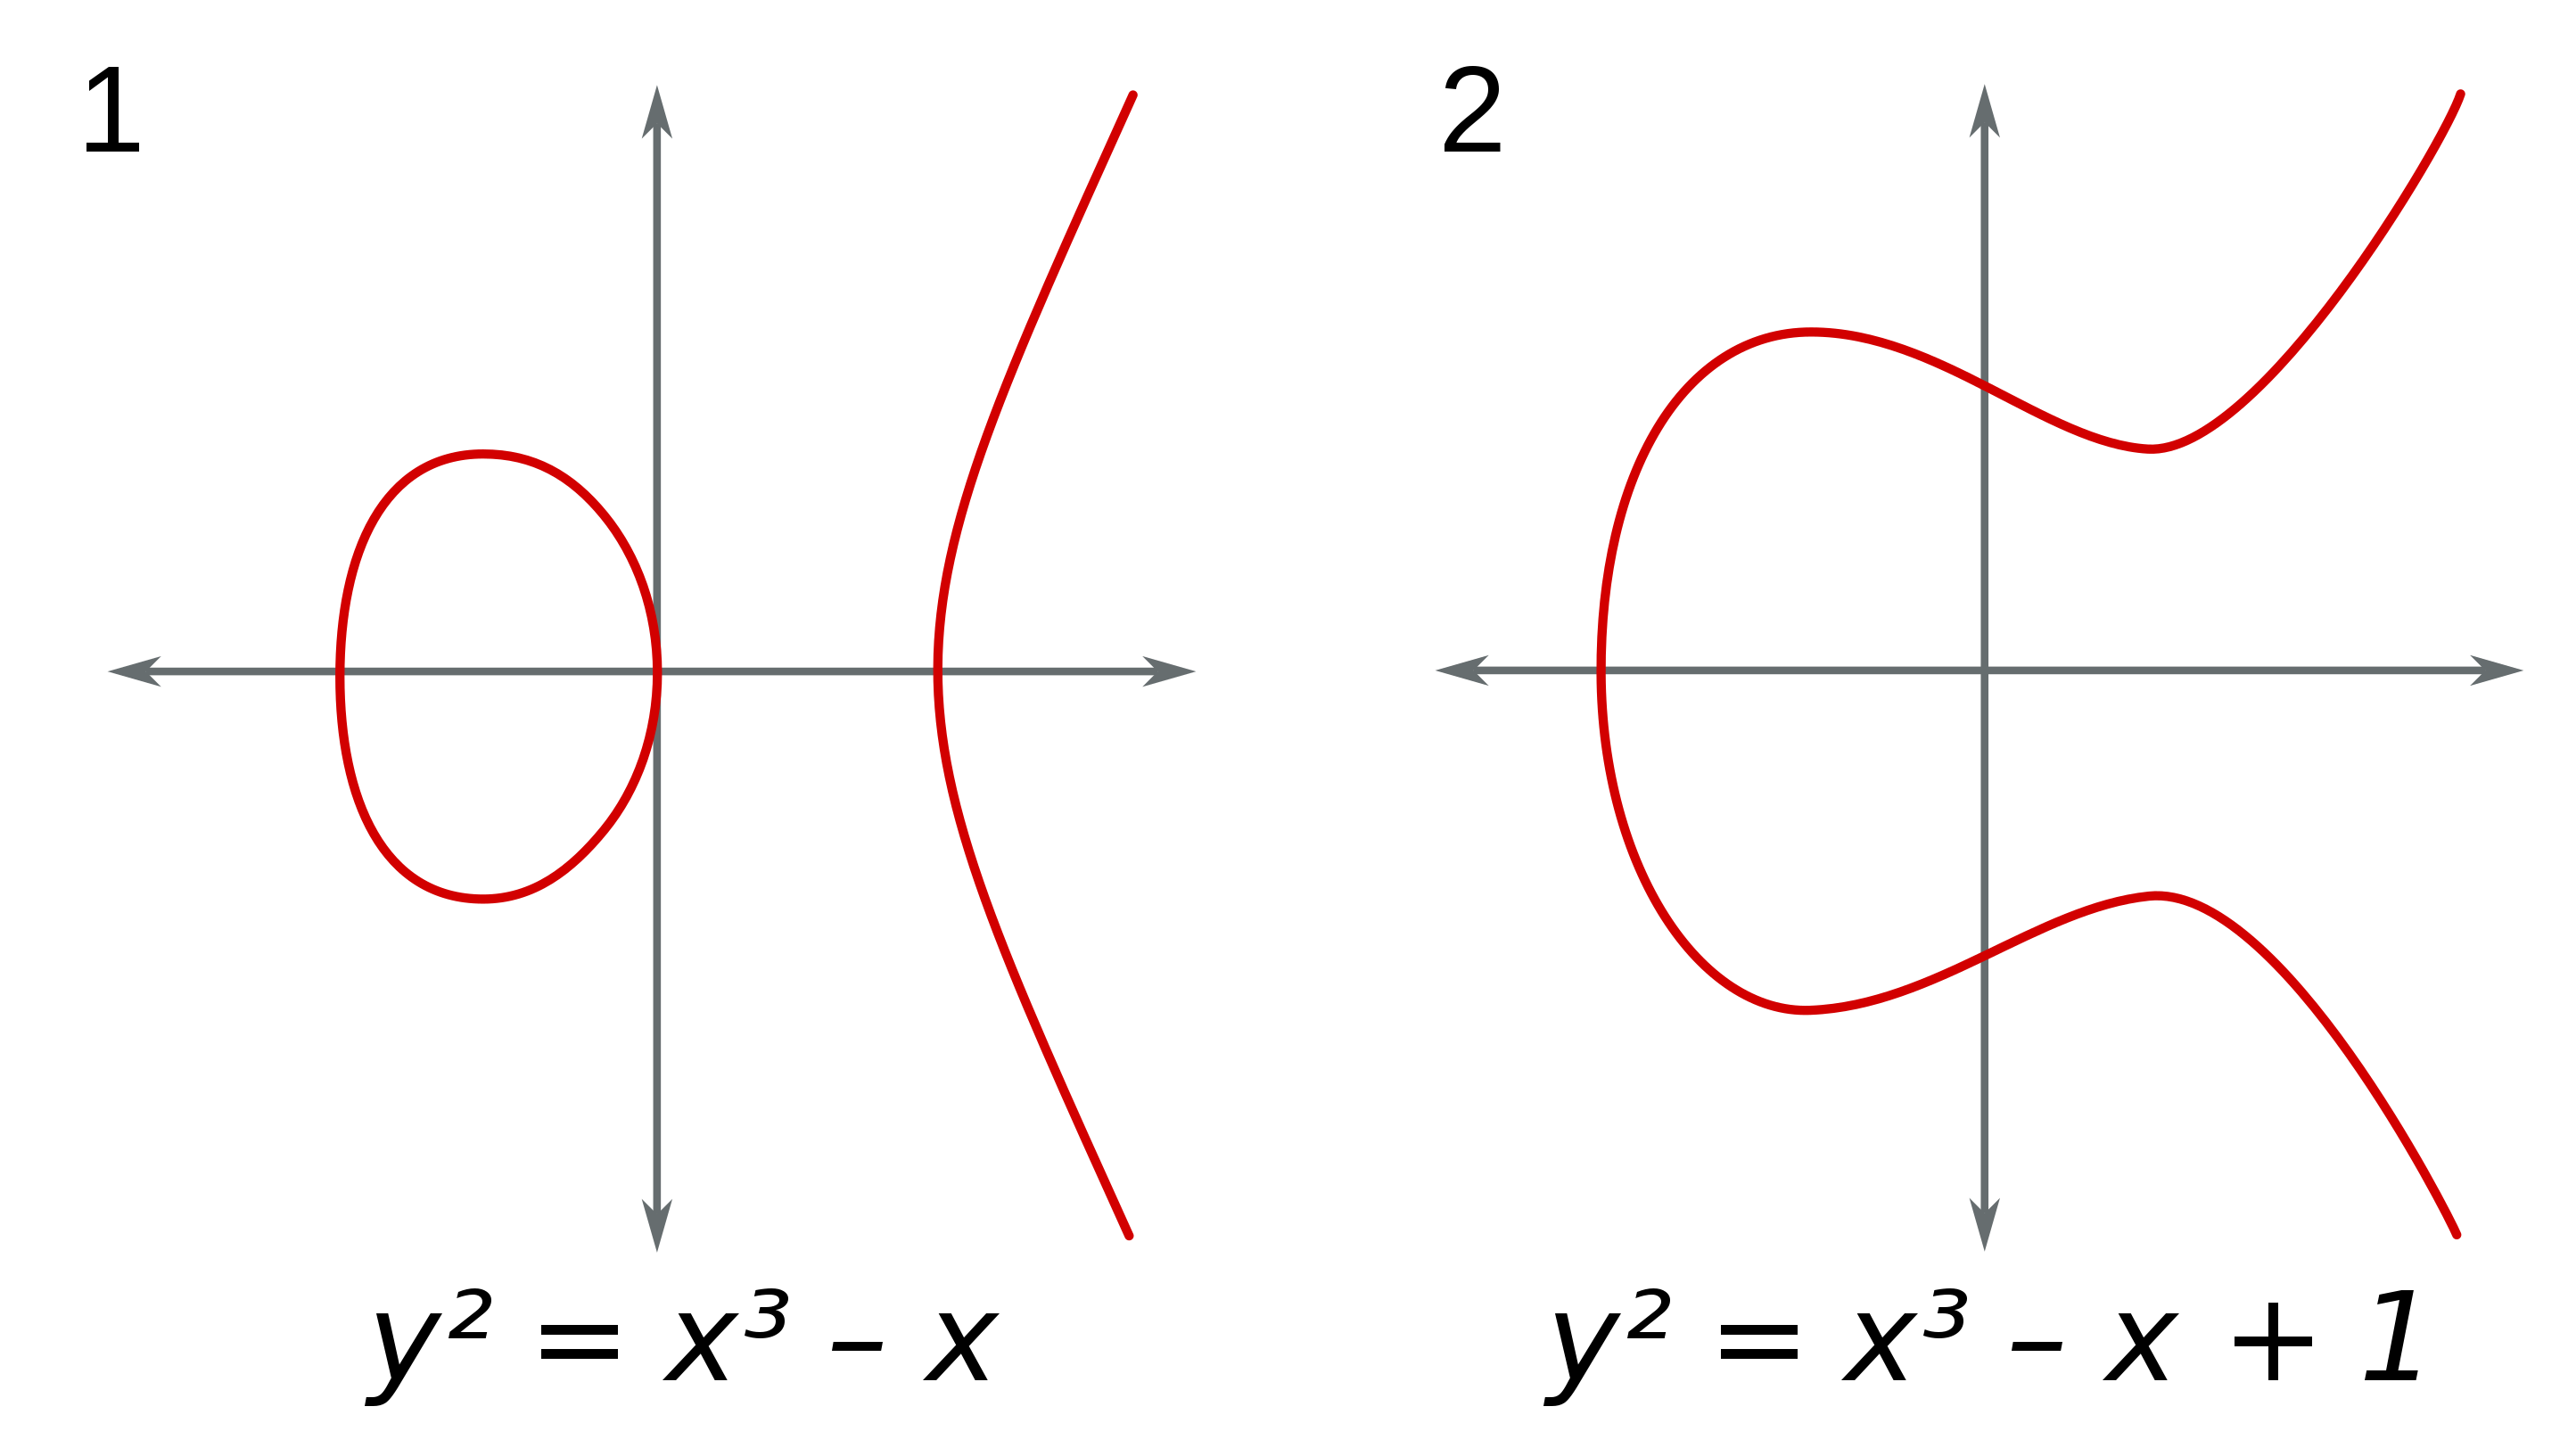
\includegraphics[width=0.8\textwidth]{fig_ec_examples.png}
\mbox{\tiny source: \url{https://commons.wikimedia.org/wiki/File:ECClines-3.svg}}
\mbox{\tiny licence: \url{https://creativecommons.org/licenses/by-sa/3.0/legalcode}, no changes were made.}
\end{figure}
\end{frame}

\begin{frame}{ Example : $\dim A=1$ elliptic curves }
Group law in pictures, over $k=\R$:
\begin{figure}[h]
\label{fig:add_law}
\centering
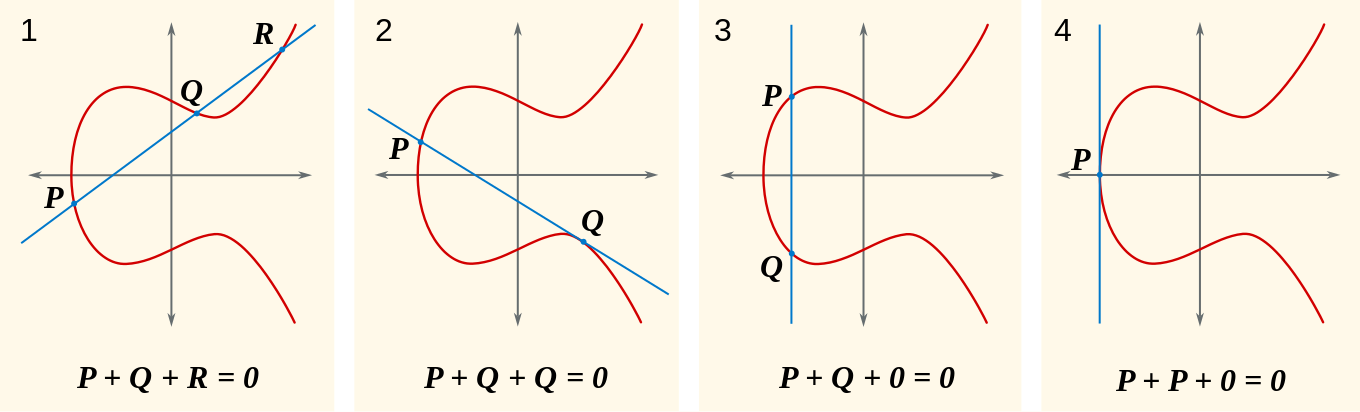
\includegraphics[width=\textwidth]{fig_ec_group_law.png}
\mbox{\tiny source: \url{https://commons.wikimedia.org/wiki/File:ECClines.svg}}
\mbox{\tiny licence: \url{https://creativecommons.org/licenses/by-sa/3.0/legalcode}, no changes were made.}
\end{figure}
\end{frame}

\begin{frame}{ In higher dimension }
\begin{itemize}\setlength\itemsep{1em}
	\item If $\dim A >1$ we have \green{equations} ($A$ is projective!)...
	\pause \item ...but in general they are really complicated.
	\pause \item In 1990 Flynn: equations for a ``general'' \red{abelian surface} (in $\Char(k) \neq 2,3,5$).

	\pause \item they look like this:
\end{itemize}
\end{frame}

{
\setbeamercolor{background canvas}{bg=}
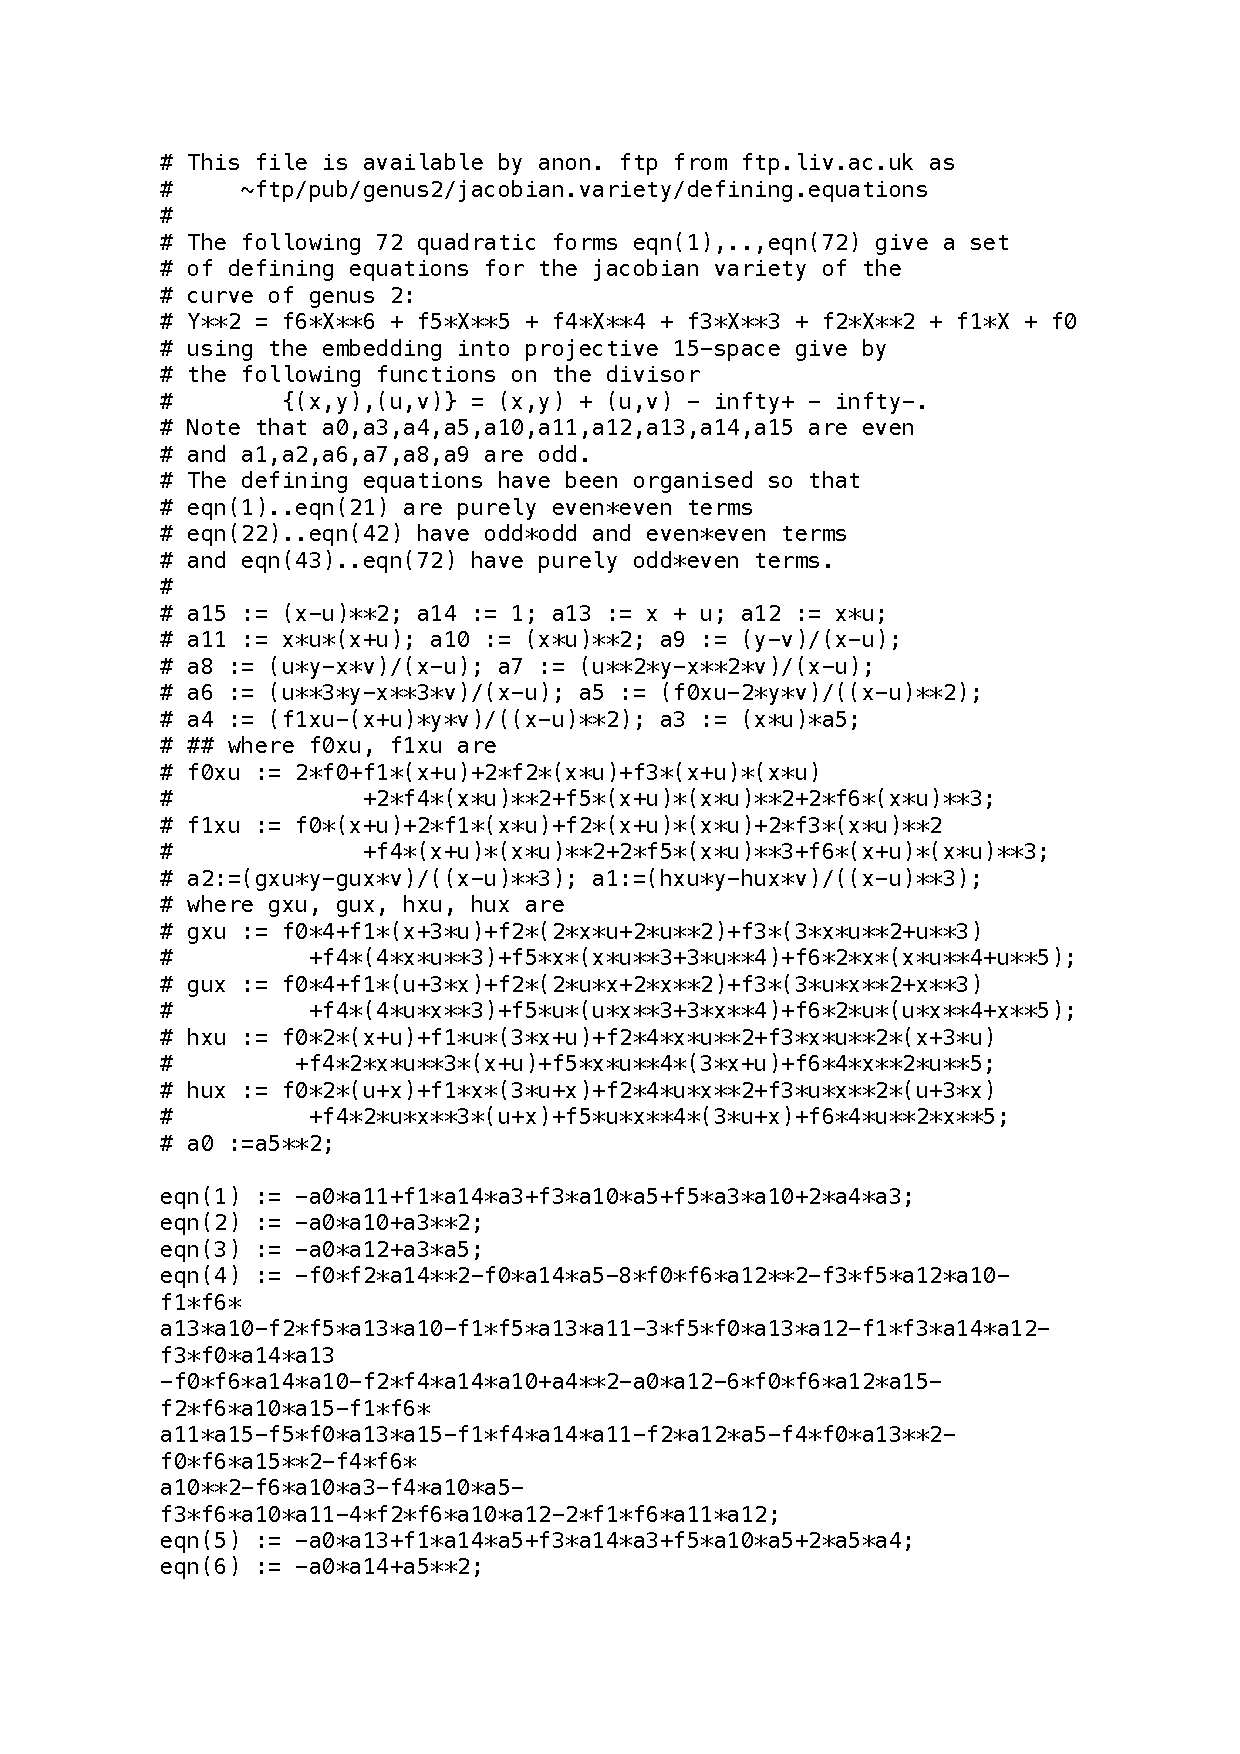
\includepdf[pages={1-2}, nup=2x1]{defining_equations.pdf}
}

{
\setbeamercolor{background canvas}{bg=}
\includepdf[pages={3-4}, nup=2x1]{defining_equations.pdf}
}

{
\setbeamercolor{background canvas}{bg=}
\includepdf[pages={5-6}, nup=2x1]{defining_equations.pdf}
}

\begin{frame}{ In higher dimension }
\begin{itemize}\setlength\itemsep{2em}
	\item \red{$72$ equations} in  \red{$16$ variables}.....
	\item (reference: Flynn-Cassels ``Prolegomena to a Middlebrow Arithmetic of Curves of Genus 2'')
\end{itemize}
\end{frame}

\begin{frame}{ Other representations }
\begin{itemize}
	\item \red{Jacobian} of curves (up to $g=3$):
	\begin{align*}
		\set{\parbox{8.6em}{proper smooth genus $g$ curves over $k$}} & \longrightarrow \set{\parbox{7em}{princ.~pol.~AVs of dim.~$g$ over $k$}} \\
			C & \longmapsto \Jac(C):=\Pic^0_k(C)
	\end{align*}
\end{itemize}
\pause Also:
	\begin{itemize}
		\pause \item \green{Prym} varieties (up to $g=5$)
		\pause \item \blue{Kummer} varieties (more compact representation)
	\end{itemize}
\end{frame}

\begin{frame}{ Over $k=\C$ }
\begin{itemize}
	\item An abelian variety over $\C$ of dimension $g$ is a \green{complex torus}.
	\[ A(\C) \simeq \faktor{\C^g}{L} \]
	where $L$ is a \green{lattice}, that is, a free sub-$\Z$-module of $\C^g$ of rank $2g$.
	\pause \item Tori (coming from AVs) admit a \blue{Riemann form}.
	\pause \item We have an \red{equivalence of categories}:
	\[
      \set{ \text{abelian varieties $/\C$} } \longleftrightarrow 
      \set{\parbox[c]{10em}{$\C^g/L$ with $L\simeq \Z^{2g}$ with\\eq.cl.~of Riemann form}}
 	\]
\end{itemize}
\end{frame}

\begin{frame}{ Over $\F_q$ }
\begin{itemize}
	\item In $\Char(k)=$ \red{$p$} such an equivalence \red{cannot hold}.
	\item There are supersingular elliptic curves with quaternionic endomorphism algebra.
	\item In particular over $\F_q$, we need to \green{restrict} ourselves to sub-categories.
	\item There are \blue{various functors}:
	\begin{itemize}
	    \item Deligne : ordinary AVs over any $\F_q$
	    \item Centeleghe-Stix : AVs with no real primes over prime fields $\F_p$
	    \item ``Serre'': AVs isogenous to power of ``some'' elliptic curves.
	\end{itemize}
\end{itemize}
\end{frame}

%\begin{frame}{ Deligne's equivalence }
%\begin{theorem}[Deligne '69]
%Let $q=p^r$, with $p$ a prime.
%There is an \red{equivalence of categories}:
%\[ \begin{array}{cc}
%\set{\text{ {\bf Ordinary} abelian varieties over } \F_q } 	& A \\
%\pause \updownarrow											& \downmapsto \\
%\set{\parbox[p]{19em}{pairs $(T,F)$, where $T\simeq_\Z \Z^{2g}$ and $T\overset{F}{\to} T$ s.t.\\
%- $F\otimes \Q$ is semisimple\\
%- the roots of $\Char_{F\otimes\Q}(x)$ have abs. value $\sqrt{q}$\\
%- \textbf{half of them are $p$-adic units}\\
%- $\exists V:T\to T$ such that $FV=VF=q$
%}}	& (T(A),F(A))
%\end{array} \]
%\end{theorem}
%\pause
%\begin{remark}
%\begin{itemize}
% \item If $\dim(A)=g$ then $\rk(T(A))=2g$;
% \item $\Frob(A)\rightsquigarrow F(A)$.
%\end{itemize}
%\end{remark}
%\end{frame}

\begin{frame}{My research: compute AVs up-to-isomorphism}
	\begin{itemize}
		\item Fix an \textbf{ordinary squarefree} $q$-Weil polynomial \red{$h$} :
\pause  \item by \red{Honda-Tate} theory $\rightsquigarrow \text{an isogeny class } \red{\cC_h}$.
\pause 	\item Put $K := \Q[x]/(h)=\Q[F]$.

\pause 	\item \green{Deligne's equivalence} induces:
% \vspace{-2 em}
			\begin{theorem}[M.]
			\[\begin{array}{cc}
			\faktor{\set{\text{abelian varieties over $\F_q$ in $\cC_h$}}}{\simeq} & \\
			\pause \updownarrow & \\
			\faktor{\set{ \text{fractional ideals of $\Z[F,q/F] \subset K$ } }}{\simeq} &\pause =:  \blue{\ICM(\Z[F,q/F])}\\ 
			& \blue{\text{ ideal class monoid} }
			  \end{array}\]
			\end{theorem}
%\pause \item \red{Problem: } $\Z[F,q/F]$ might not be maximal $\rightsquigarrow $ \red{non-invertible} ideals.
%\pause \item \green{Solution: } attack the problem locally and then get the global result using the action of the $\Pic$s. 
	\end{itemize}
\end{frame}

\begin{frame}{ Example}
\begin{itemize}\setlength\itemsep{1em}
 \item Let $h(x)=x^8 - 5x^7 + 13x^6 - 25x^5 + 44x^4 - 75x^3 + 117x^2 - 135x + 81$.
 \pause \item $\rightsquigarrow$ isogeny class of an simple ordinary abelian varieties over $\F_{3}$ of \green{dimension $4$}.
 \pause  \item Let $F$ be a root of $h(x)$ and put $R:=\Z[F,3/F]\subset \Q(F)$.
% \item $8$ over-orders of $R$: two of them are not Gorenstein.
 \item $\#\ICM(R) = 18 \rightsquigarrow $  \red{$18$ isom.~classes} of AV in the isogeny class.
% \item $5$ are not invertible in their multiplicator ring.
% \item $8$ classes admit principal polarizations.
% \item $10$ isomorphism classes of princ. polarized AV.
\end{itemize}
\end{frame}

\begin{frame}{Example}{}
Concretely:
{\scriptsize \begin{align*}
  \begin{split} 
  I_1 = & 2645633792595191 \Z \oplus (F + 836920075614551) \Z \oplus (F^2 + 1474295643839839)\Z \oplus\\
	& \oplus (F^3 + 1372829830503387)\Z \oplus (F^4 + 1072904687510)\Z \oplus\\
	& \oplus \frac{1}{3}(F^5 + F^4 + F^3 + 2F^2 + 2F + 6704806986143610)\Z \oplus\\
	& \oplus \frac{1}{9}(F^6 + F^5 + F^4 + 8F^3 + 2F^2 + 2991665243621169) \Z \oplus\\
	& \oplus \frac{1}{27}(F^7 + F^6 + F^5 + 17F^4 + 20F^3 + 9F^2 + 68015312518722201)\Z\\
  \end{split}\\  
  \begin{split} 
  I_7 = & 2\Z\oplus(F + 1)\Z\oplus(F^2 + 1)\Z\oplus(F^3 + 1)\Z\oplus(F^4 + 1)\Z\oplus\frac13(F^5 + F^4 + F^3 + 2F^2 + 2F + 3)\Z \oplus \\ 		      & \oplus\frac{1}{36}(F^6 + F^5 + 10F^4 + 26F^3 + 2F^2 + 27F + 45)\Z\oplus\\
	& \oplus \frac{1}{216}(F^7 + 4F^6 + 49F^5 + 200F^4 + 116F^3 + 105F^2 + 198F + 351)\Z\\
  \end{split}
  \end{align*}}
\pause $I_1$ is invertible in $R$, but $I_7$ is not invertible in $\End(I_7)$.
\end{frame}

\begin{frame}{ Math Commercials : Computations }
\begin{itemize}\setlength\itemsep{1em}
 \pause \item With ``Simons Collaboration on Arithmetic Geometry, Number Theory, and Computation''
 
 \pause \item computing on a server computer at the MIT.
 
 \pause \item Data for $\sim 700.000$ isogeny classes for various $g$ and $\F_q$.
 
 \pause \item Some are pretty \green{big}: ($> 5$ millions isomorphism classes).\\
 
 \pause \item \blue{Coming soon on the LMFDB} (\url{https://www.lmfdb.org/Variety/Abelian/Fq/})

\end{itemize}
\end{frame}

\begin{frame}{ Non-Math Commercials: Where have I been ? }
\pause \begin{itemize}\setlength\itemsep{1em}
	\item Bachelor: Universitá di Torino.
	\item Master: ALGANT (Universitá di Padova , Leiden University).
	\item \green{PhD at Stockholm University (with Jonas Bergstr\"om)}.
	\item postdoc at the Max Planck Institute for Mathemamatics in Bonn.
	\item now: postdoc at Utrecht University (with Carel Faber).
\end{itemize}
\pause If you have any question about any of these places: \red{ask away}!
\end{frame}

\begin{frame}{ }
\begin{center}
{\Large Thank you!}
\end{center}
\end{frame}

\end{document}
